\section{Wargame Scenario}
\label{sec:wargame}

The game can have up to four players, where some can be set to move in predefined patterns, so that one can get a feeling of playing against an artificial intelligence.\\ \indent
	When the application is started, the user chooses the size of the battle area, and the agents and teams are set up by the input of the generated XML-file \ref{agents_patterns}.

\begin{figure}[H]
\begin{center}
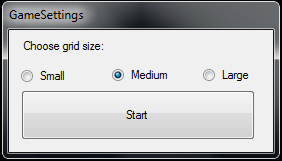
\includegraphics{Images/settings.png}
\end{center}
\caption{The player can choose between 3 diffrent sizes, small(13), medium(26) and large(46)}
\label{fig:settings}
\end{figure}

The user can type his commands in the \textit{command center}, when the user is done giveing all his commands for his round, he can press the \textit{End Turn} button to make his moves and end his round.\\ \indent
	The moves available for the user to make is \textit{up}, \textit{down}, \textit{left} and \textit{right} (one coordinate at a time), and it is also possible to move several grids with an agent, if you select the agent and type the coordinates you want the agent to move to.\\ \indent
  When a collision between agents from opposing teams occur, a random function is called, deciding which agent wins the fight, favoring the unit with the highest rank.
	
\begin{figure}[H]
\begin{center}
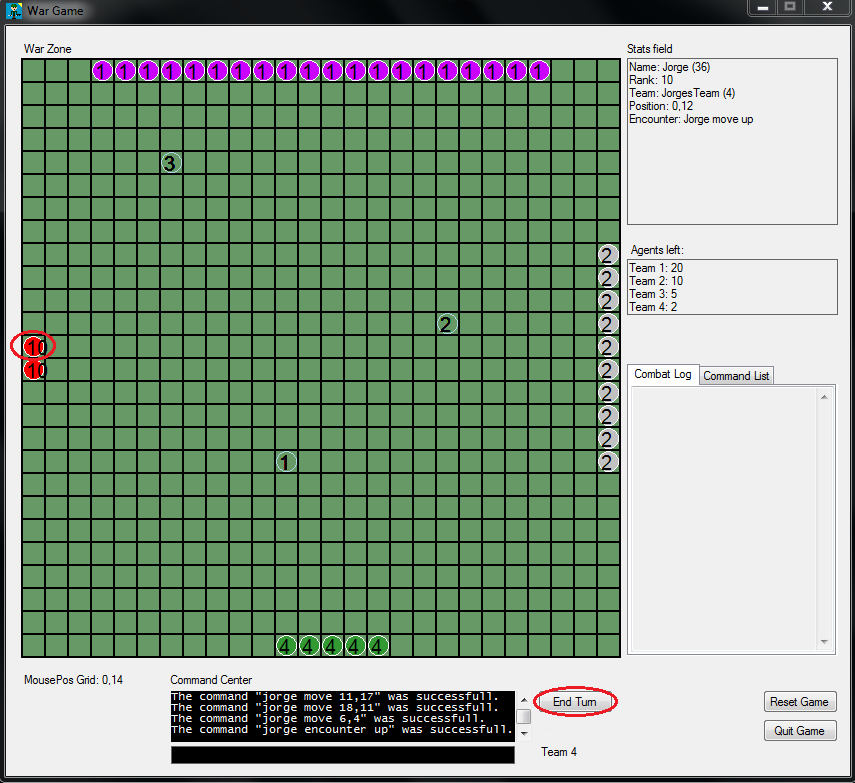
\includegraphics[scale=0.6]{Images/ex_com.png}
\end{center}
\caption{Example of an execution of a move-by-coordinate command. The user type the command \texttt{pink1 MOVE 14,3} and press \textit{Execute}. For more about the commands, see appendix \ref{actiongrammar}.}
\label{fig:ex_com}
\end{figure}

\subsection{Agents and Action Patterns}
\label{agents_patterns}

The XML-document, which is loaded when the game initialized, sets the up the teams with number of players, division into squads, and rank of the agents. Also the action patterns are set by the XML-document.